\documentclass{article}
\usepackage{graphicx} % Required for inserting images
\providecommand{\keywords}[1] {
\small \textbf{\textit{Keywords---}} #1
}

\title{A study on the use of deep reinforcement learning in games development and its role in in-game character behavior and decision-making.}
\author{Prajwol Devkota }
\date{December 10, 2023}

\begin{document}

\maketitle
\begin{abstract}
The abstract section provides a summary of the topic, which is \textbf{how can deep reinforcement learning be used in game development, and its role in in-game character behavior and decision-making.} 
\end{abstract}

\keywords {The keywords are the important words found in the research papers, which help other researchers find your paper when researching the relevant topic.}
 
\section{INTRODUCTION}

Artificial Intelligence (AI) has seen immense progress in recent years. It is both a thriving research field featuring an increasing number of important research areas and a core technology for an increasing number of application areas. In addition to algorithmic innovations, the rapid progress in AI is often attributed to increasing computational power due to hardware advancements. The success stories of AI can be experienced in our daily lives through its many practical applications. AI advances have enabled a better understanding of images and speech, emotion detection, self-driving cars, web searching, AI-assisted creative design, and game-playing,
among many other tasks; for some of these tasks, machines have reached human-level status or beyond.

There is, however, a difference between what machines can do well and what humans are good at. In the early days of AI, researchers envisaged computational systems that would exhibit aspects of human intelligence and achieve human-level problem-solving or decision-making skills. These problems were presented to the machines as a set of formal mathematical notions within rather narrow and controlled spaces, which could be solved by some form of symbol manipulation or search in symbolic space. The highly formalized, symbolic representation allowed AI to succeed in many cases.

Over the years the focus of much AI research has shifted to tasks that are relatively simple for humans to do but are hard for us to describe how to do, such as remembering a face or recognizing our friend’s voice over the phone. As a result, AI researchers began to ask questions such as: How can AI detect and express emotion? How can AI educate people, and be creative or artistically novel? How can AI play a game it has not seen before? How can AI learn from a minimal number of trials? How can AI feel guilt? All these questions pose serious challenges to AI and correspond
to tasks that are not easy for us to formalize or define objectively. Perhaps surprisingly (or unsurprisingly after the fact), tasks that require relatively low cognitive effort from us often turn out to be much harder for machines to tackle. Again, games have provided a popular domain to investigate such abilities as they feature aspects of a subjective nature that cannot be formalized easily. These include, for
instance, the experience of play or the creative process of game design\cite{schell2008art}.

\subsection{A BRIEF HISTORY OF AI AND GAMES}

Artificial intelligence (AI) and games have a long history, with early pioneers of computer science developing game-playing programs to test the capabilities of computers. The focus of early research was on classic board games like Chess and Checkers. Significant milestones include the development of the Minimax algorithm by Alan Turing, the first software to master a game (Tic-Tac-Toe) by A. S. Douglas, and the invention of reinforcement learning by Arthur Samuel for playing Checkers. The successes of AI in classic board games, such as Deep Blue's victory over Garry Kasparov in Chess and AlphaGo's triumph in the game of Go, marked important milestones in game-playing AI. In recent years, there has been a growing research community applying AI to a variety of games, including video games. This has led to achievements such as Google DeepMind's algorithms learning to play Atari 2600 games at a super-human level and the use of AI for procedural content generation in games like Diablo III and No Man’s Sky. AI has also been used to analyze games and model players, and there has been a focus on developing believable agents in games. The application of AI in games continues to evolve, with ongoing research and development in this field\cite{yannakakis2018artificial}.

\section{ARTIFICIAL INTELLIGENCE}
To understand the use of deep reinforcement learning in game development, one must first know about Deep Learning and Reinforcement Learning, which comes under Machine Learning, which is an approach to achieving Artificial Intelligence. In this paper, a brief description is given about all these fields is given before describing Deep Reinforcement Learning.

According to the father of Artificial Intelligence, John McCarthy, it is \textit{“The science and engineering of making intelligent machines, especially intelligent computer programs”.}

Artificial Intelligence (AI) is the ability of a machine or a computer program to think and learn. The concept of AI is based on the idea of building machines capable of thinking, acting, and learning like humans.

AI is accomplished by studying how the human brain thinks, and how humans learn, decide, and work while trying to solve a problem, and then using the outcomes of this study as a basis for developing intelligent software and systems.
\subsection{Goals of AI}

\begin{itemize}
\item To Create Expert Systems - The systems that exhibit intelligent behavior, learn, demonstrate, explain, and advise its users.
\item To Implement Human Intelligence in Machines - Creating systems that understand, think, learn, and behave like humans.
\end{itemize}

\subsection{Programming Without and With AI}
The difference between programming with AI and without AI is given below in Fig. \ref{fig: the difference between programming without AI and with AI.}

\begin{figure}[h]
\centering
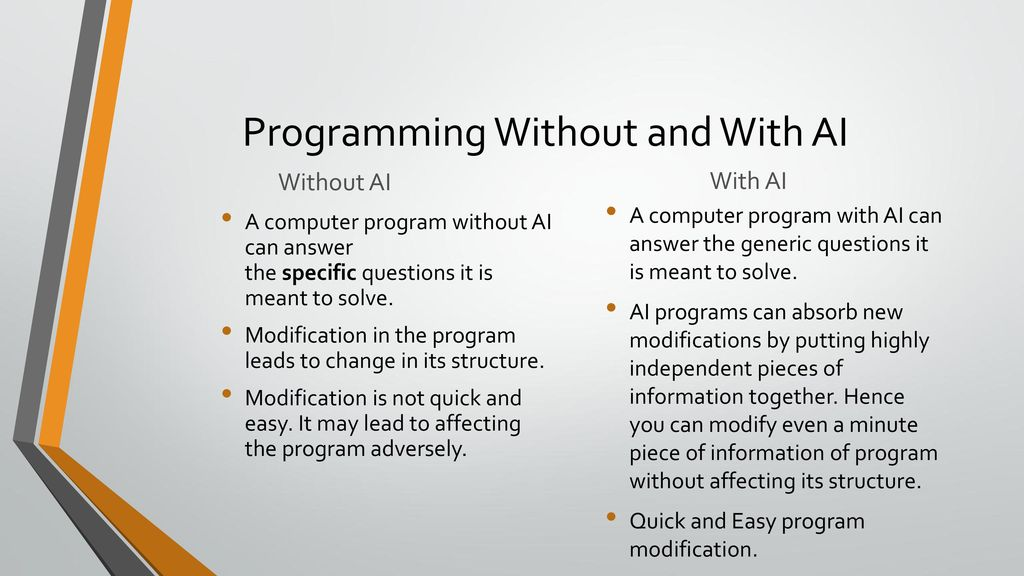
\includegraphics[width=1\textwidth]{image1.jpg}
\caption{The difference between the programming without AI and with AI\cite{Deshai_2017}.}
\label{fig: the difference between programming without AI and with AI.}
\end{figure}

\subsection{MACHINE LEARNING}
Machine Learning is a large sub-field of AI dealing with the field of study that gives computers the ability to learn without being explicitly programmed. This means a single program, once created, will be able to learn how to do some intelligent activities outside the notion of programming. This contrasts with purpose-built programs whose behavior is defined by hand-crafted heuristics that explicitly and statically define their behavior. So, Machine Learning is an approach to achieve Artificial Intelligence.

Machine learning combines data with statistical tools to predict an output. This output is then used by corporations to make actionable insights. Machine learning is closely related to data mining and Bayesian predictive modeling. The machine receives data as input, and uses an algorithm to formulate answers.

\subsection{Machine Learning vs Traditional Programming}
Traditional programming differs significantly from machine learning. In traditional programming, a programmer codes all the rules in consultation with an expert in the industry for which the software is being developed. Each rule is based on a logical foundation; the machine will execute an output following the logical statement. When the system grows complex, more rules need to be written. It can quickly become unsustainable to maintain.

Machine learning is supposed to overcome this issue. The machine learns how the input and output data are correlated and it writes a rule. The programmers do not need to write new rules each time there is new data. The algorithms adapt in response to new data and experiences to improve efficacy over time.

\begin{figure}[h]
\centering
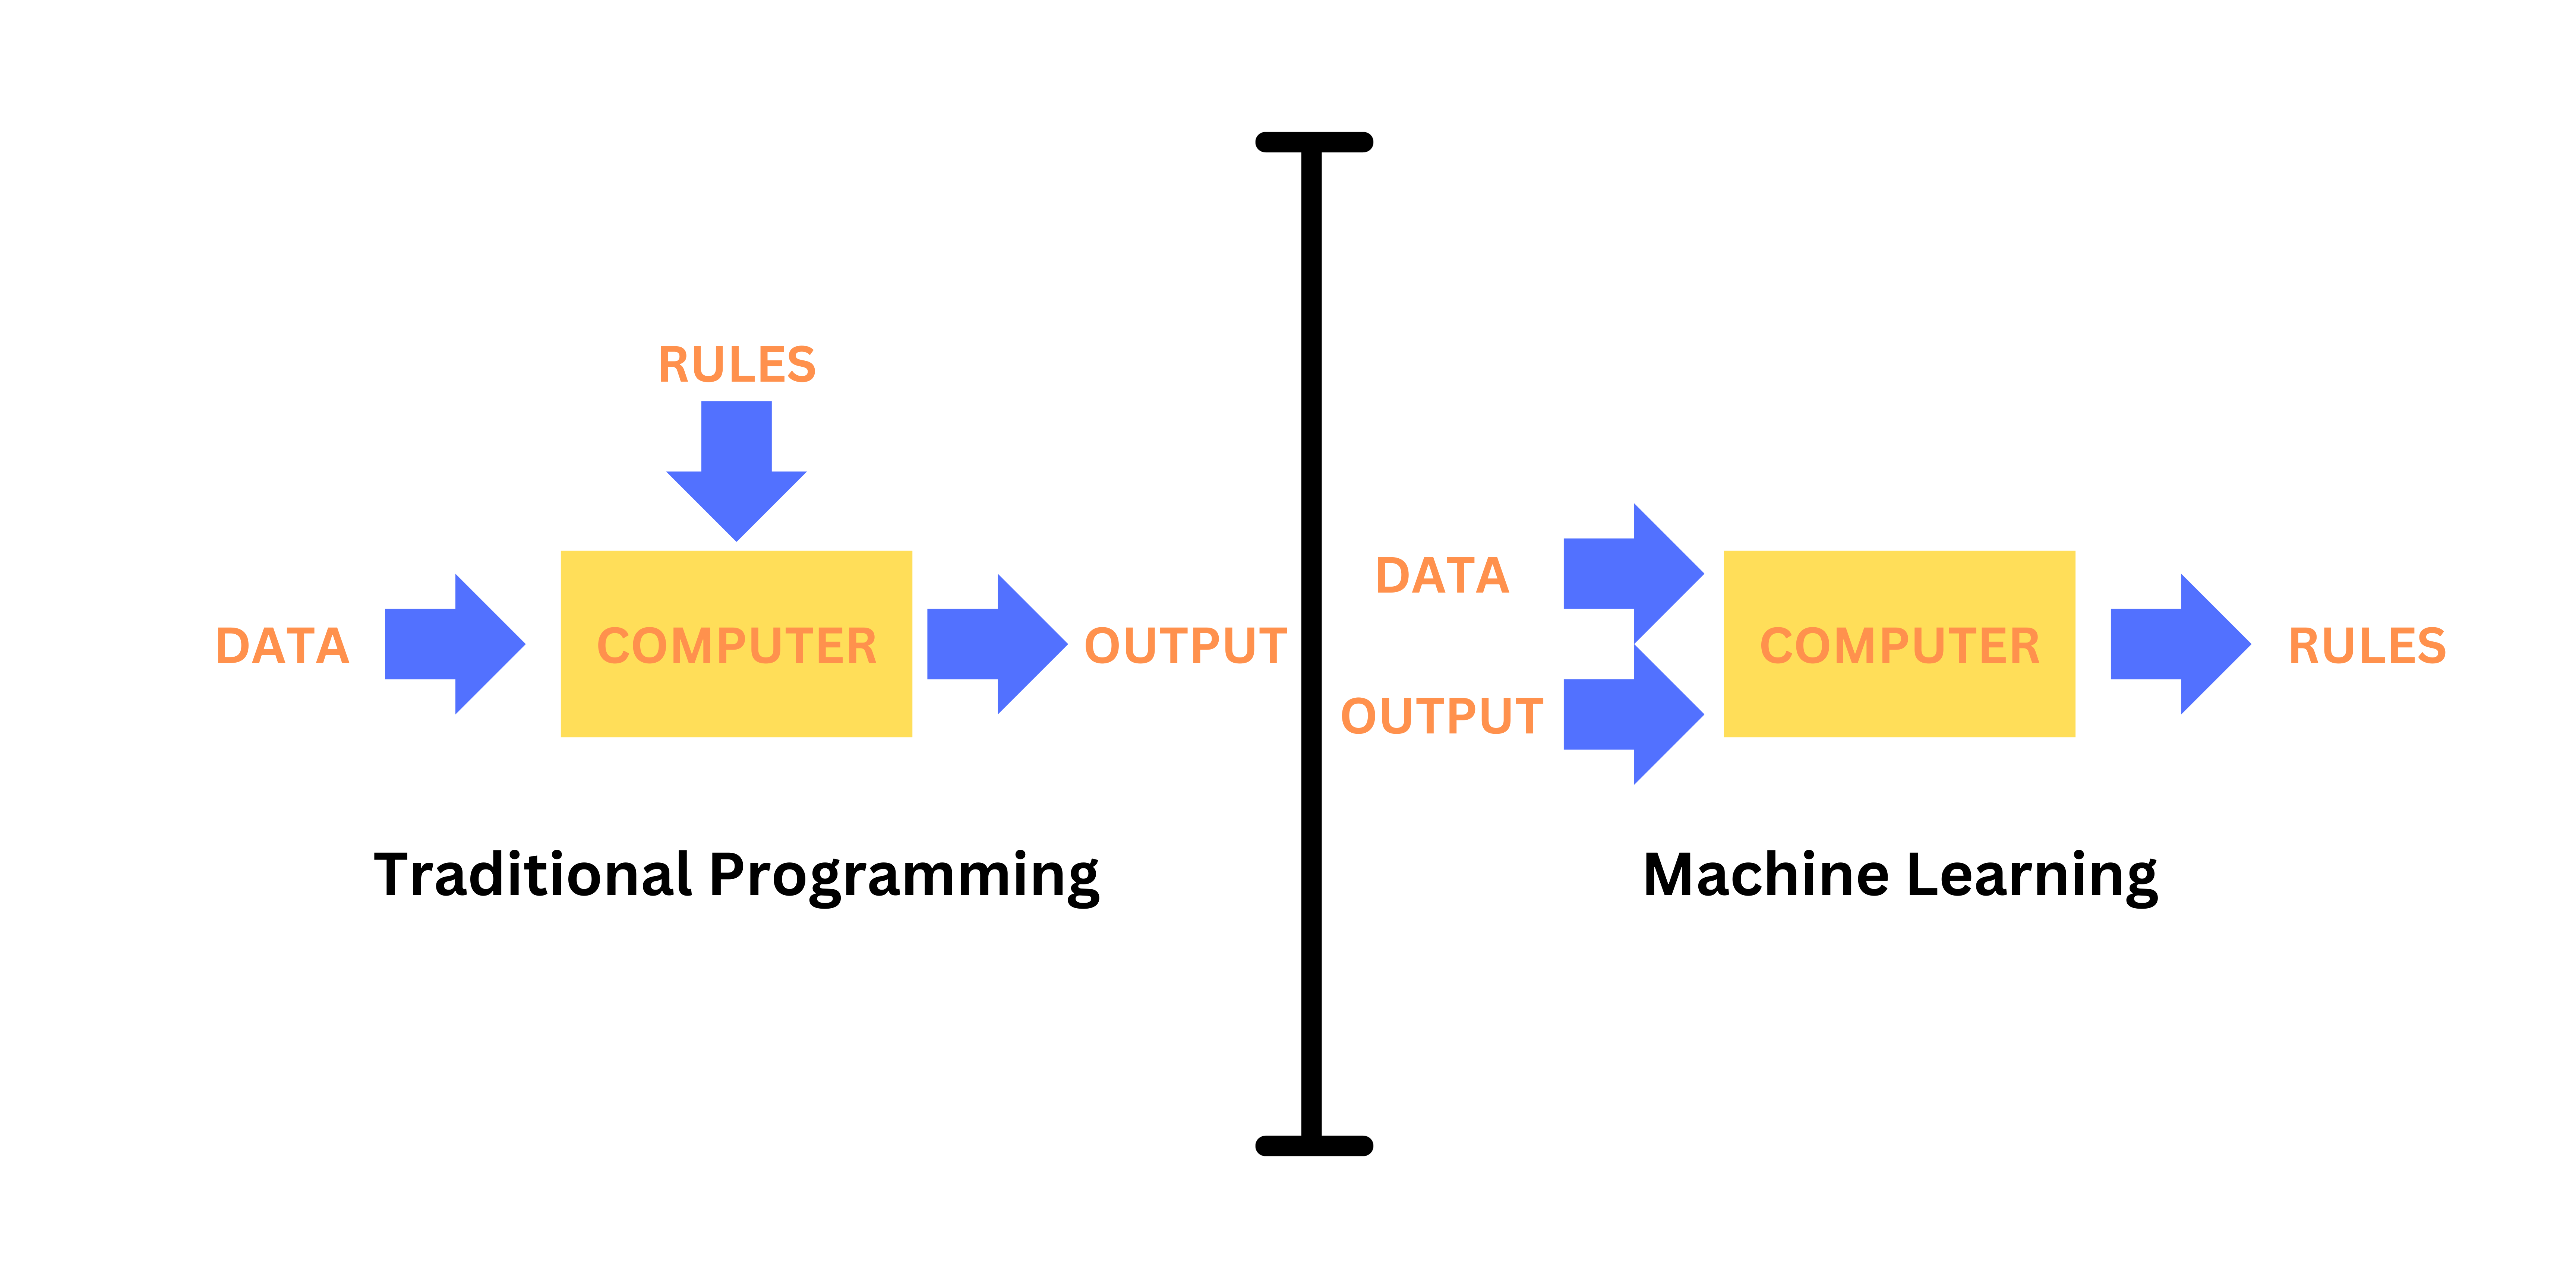
\includegraphics[width=1\textwidth]{image2.png}
\caption{The traditional programming manual process whereas in machine learning the input data and output are fed to an algorithm to create a program.}
\label{fig: the traditional programming vs machine learning.}
\end{figure}

\subsection{Types of Machine Learning}
Machine learning involves showing a large volume of data to a machine so that it can learn and make predictions, find patterns, or classify data. The three machine learning types are supervised, unsupervised, and reinforcement learning.

\begin{itemize}
\renewcommand\labelitemi{--}
\item \textbf{Supervised learning} is typically the task of machine learning to learn a function that maps an input to an output based on sample input-output pairs \cite{han2022data}. It uses labeled training data and a collection of training examples to infer a function. Supervised learning is carried out when certain goals are identified to be accomplished from a certain set of inputs \cite{sarker2020cybersecurity}, i.e., a task-driven approach. The most common supervised tasks are “classification” that separates the data, and “regression” that fits the data. For instance, predicting the class label or sentiment of a piece of text, like a tweet or a product review, i.e., text classification, is an example of supervised learning.

\item \textbf{Unsupervised learning} analyzes unlabeled datasets without the need for human interference, i.e., a data-driven process \cite{han2022data}. This is widely used for extracting generative features, identifying meaningful trends and structures, groupings in results, and exploratory purposes. The most common unsupervised learning tasks are clustering, density estimation, feature learning, dimensionality reduction, finding association rules, anomaly detection, etc.

\item \textbf{Reinforcement learning} is a type of machine learning algorithm that enables software agents and machines to automatically evaluate the optimal behavior in a particular context or environment to improve its efficiency, i.e., an environment-driven approach\cite{kaelbling1996reinforcement}. This type of learning is based on reward or penalty, and its ultimate goal is to use insights obtained from environmental activists to take action to increase the reward or minimize the risk \cite{mohammed2016machine}. It is a powerful tool for training AI models that can help increase automation or optimize the operational efficiency of sophisticated systems such as robotics, autonomous driving tasks, manufacturing, and supply chain logistics, however, not preferable to use it for solving basic or straightforward problems.
\end{itemize}

\section{REINFORCEMENT LEARNING}
Reinforcement learning (RL) is learning what to do, given a situation and a set of possible actions to choose from, in order to maximize a reward. The learner, which we will call agent, is not told what to do, he must discover this by himself through interacting with the environment. The goal is to choose its actions in such a way that the cumulative reward is maximized. So, choosing the best reward now, might not be the best decision, in the long run. That is greedy approaches might not be optimal.

Reinforcement Learning is an approach where an agent learns how to behave in a environment by performing actions and seeing the results. Reinforcement learning is connected to applications for which the algorithm must make decisions and the decisions bear consequences. The goal is defined by maximisation of expected cumulative reward.

The algorithm presents a state, depending on the input data in which a user rewards or punishes the algorithm for the action the algorithm took. The algorithm learns from the reward/punishment and updates itself, this continues.

\subsection{Components of Reinforcement learning}
\begin{itemize}
\renewcommand\labelitemi{--}
\item \textbf{Agent}  Agent (A) takes actions that affect the environment. Citing an example, the machine learning to play chess is the agent.
\item \textbf{Action} It is the set of all possible operations/moves the agent can make. The agent makes a decision on which action to take from a set of discrete actions (a).
\item \textbf{Environment} All actions that the reinforcement learning agent makes directly affect the environment. Here, the board of chess is the environment. The environment takes the agent's present state and action as information and returns the reward to the agent with a new state.
For example, the move made by the bot will either have a negative/positive effect on the whole game and the arrangement of the board. This will decide the next action and state of the board.
\item \textbf{State} A state (S) is a particular situation in which the agent finds itself.
\item \textbf{Reward} (R) The environment gives feedback by which we determine the validity of the agent’s actions in each state. It is crucial in the scenario of Reinforcement Learning where we want the machine to learn all by itself and the only critic that would help it in learning is the feedback/reward it receives.

For example, in a chess game scenario it happens when the bot takes the place of an opponent's piece and later captures it.
\item \textbf{Discount factor} Over time, the discount factor modifies the importance of incentives. Given the uncertainty of the future it’s better to add variance to the value estimates. Discount factor helps in reducing the degree to which future rewards affect our value function estimates.
\item \textbf{Policy} ($\pi$) It decides what action to take in a certain state to maximize the reward.
\item \textbf{Value} (V) It measures the optimality of a specific state. It is the expected discounted rewards that the agent collects following the specific policy.
\item \textbf{Q-value or action-value} Q Value is a measure of the overall expected reward if the agent (A) is in state (s) and takes action (a), and then plays until the end of the episode according to some policy ($\pi$).
\end{itemize}

\begin{figure}
\centering
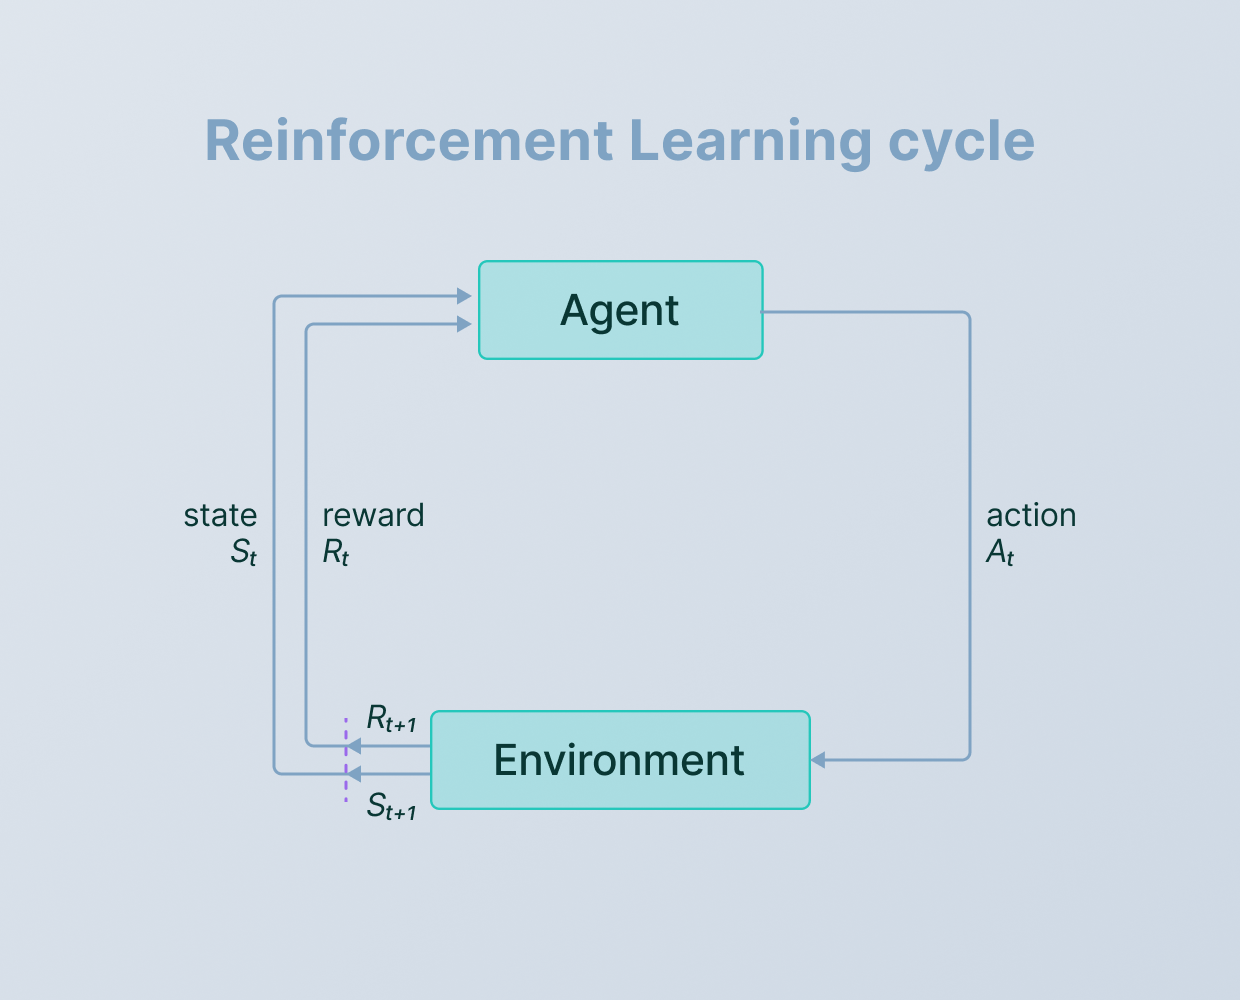
\includegraphics[width=1\textwidth]{image3.png}
\caption{Agent-environment interaction where the agent receives the rewards upon actions that lead to desired states \cite{sutton2018reinforcement}.}
\label{fig: Agent-environment interaction in RL.}
\end{figure}

There is an agent and an environment. The environment gives the agent a state. The agent chooses an action and receives a reward from the environment along with the new state. This learning process continues until the goal is achieved or some other condition is met.

\section{DEEP LEARNING}
Deep Learning comes in the area of Neural Networks.
Within the machine learning fields, there is an area often referred to as brain-inspired computation. Human brain is one of the best ‘machines’ we know for learning and solving problems. The brain-inspired technique is indeed inspired by how our human brain works. It is believed that the main computational element of our brain is neuron. The complex connected network of neurons forms the basis of all the decisions made based on the various information gathered. This is exactly what Artificial Neural Network technique does.

Within the domain of neural networks, there is an area called Deep Learning (DL), in which neural networks have more than three layers, i.e. more than one hidden layer. These neural networks used in Deep learning are called Deep Neural Networks (DNNs). DL algorithms are similar to how nervous system structured where each neuron connected each other and passing information. DL models work in layers and a typical model at least have three layers and each layer accepts the information from previous and pass it on to the next one.

Deep learning models tend to perform well with amount of data whereas old machine learning models stops improving after a saturation point.
\begin{figure}[h]
\centering
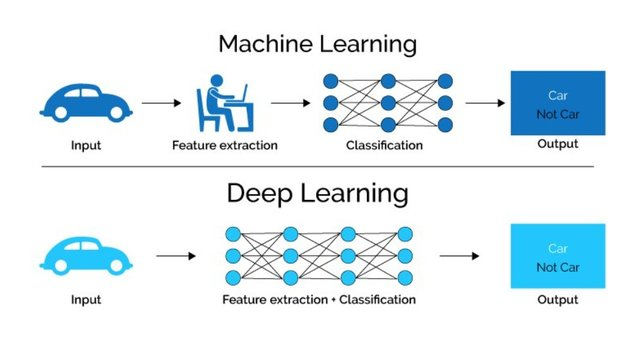
\includegraphics[width=1\textwidth]{image4.png}
\caption{Machine learning and deep learning algorithms strategies overview \cite{thakur2021fundamentals}.}
\label{fig: Machine learning and deep learning algorithms.}
\end{figure}

\section{DEEP REINFORCEMENT LEARNING}
Deep Reinforcement Learning is a new research track within the field of Machine Learning. While neural networks are responsible for recent breakthroughs in problems like computer vision, machine translation and time series prediction — they can also combine with reinforcement learning algorithms to create something astounding like AlphaGo \cite{silver2016mastering}. Reinforcement algorithms that incorporate deep learning can beat world champions at the game of Go as well as human experts playing numerous Atari video games \cite{mnih2015human}. While that may sound trivial, it’s a vast improvement over their previous accomplishments, and the state of the art is progressing rapidly.

Like a human, our agents learn for themselves to achieve successful strategies that lead to the greatest long-term rewards. This paradigm of learning by trial-and-error, solely from rewards or punishments, is known as Reinforcement Learning (RL). Also like a human, agents construct and learn their own knowledge directly from raw inputs, such as vision, without any hand-engineered features or domain heuristics. This is achieved by Deep Learning of neural networks. Many of the successes in DRL have been based on scaling up prior work in RL to high-dimensional problems. This is due to the learning of low-dimensional feature representations and the powerful function approximation properties of neural networks. By means of representation learning, DRL can deal efficiently with the curse of dimensionality, unlike tabular and traditional nonparametric methods \cite{bengio2013representation}. For instance, convolutional neural networks (CNNs) can be used as components of RL agents, allowing them to learn directly from raw, high-dimensional visual inputs. The use of deep learning is most useful in problems with high-dimensional state space. This means that with deep learning, Reinforcement Learning is able to solve more complicated tasks with lower prior knowledge because of its ability to learn different levels of abstractions from data.

To use reinforcement learning successfully in situations approaching real-world complexity, however, agents are confronted with a difficult task: they must derive efficient representations of the environment from high-dimensional sensory inputs, and use these to generalize past experience to new situations. This makes it possible for machines to mimic some human problem-solving capabilities, even in high-dimensional space, which only a few years ago was difficult to conceive.

\subsection{Applications}
DRL has gained significant traction in recent years due to its remarkable ability to solve complex problems, particularly those involving sequential decision-making and high-dimensional continuous action spaces. Its applications have expanded across various domains, as shown in Table \ref{tab: DRL applications across various domains.} 


\begin{table}
\centering
\begin{tabular}{|c|c|} \hline
    \textbf{Domains}& \textbf{Application}\\ \hline 
         Computer systems& Resources management, security\\ \hline 
         Education& Educational games, recommendation, estimation\\ \hline 
         Transportation&Traffic control\\ \hline 
         Games Development& Board games, card games, video games\\ \hline 
         Robotics& Sim-to-real, control\\ \hline 
         Science, Engineering, Art& Math, Physics, music, animation\\ \hline 
         Business management& Recommendation, customer management\\ \hline 
         Computer vision& Recognition, detection, perception\\ \hline 
         NLP& Sequence generation, translation, dialogue\\\hline
    \end{tabular}
    \caption{DRL applications across various domains \cite{li2017deep}.}
    \label{tab: DRL applications across various domains.}
\end{table}

\section{APPLICATIONS OF DRL IN GAMES DEVELOPMENT}


\section{CHALLENGES AND LIMITATIONS}
\section{CONCLUSION AND DISCUSSION}
\section{Acknowledgments}
The acknowledgments section gives recognition to the individuals or organizations who have contributed to the research by providing support, and guidance during the research process.
\newpage
\bibliographystyle{apalike}
\bibliography{references}
\end{document}
